\documentclass[titlepage, 11pt]{article}
\usepackage{fullpage}
\usepackage[T1]{fontenc}
\usepackage[utf8]{inputenc}
\usepackage{lmodern}
\usepackage{graphicx}
\graphicspath{ {figures/} }
\usepackage{amsmath}
\usepackage[english]{babel}
\usepackage{csquotes}
\usepackage{enumerate}
\usepackage[margin = 2 cm]{geometry}
\usepackage{longtable}
\usepackage{setspace}
\usepackage{glossaries}
\usepackage{amsfonts}
\usepackage{array}
\usepackage[titletoc,toc,title]{appendix}
\usepackage{biblatex}
\bibliography{11.bib}


\newcommand\Exp{\mathbb{E}\AverX}


\newcolumntype{L}[1]{>{\raggedright\let\newline\\\arraybackslash\hspace{0pt}}m{#1}}
\newcolumntype{C}[1]{>{\centering\let\newline\\\arraybackslash\hspace{0pt}}m{#1}}
\newcolumntype{R}[1]{>{\raggedleft\let\newline\\\arraybackslash\hspace{0pt}}m{#1}}
\makeatletter
\newcommand*{\rom}[1]{\expandafter\@slowromancap\romannumeral #1@}
\makeatother
%\renewcommand{\baselinestretch}{1.5}
\makeglossaries
\begin{document}
\begin{titlepage}


\newcommand{\HRule}{\rule{\linewidth}{0.5mm}} % Defines a new command for the horizontal lines, change thickness here

\center % Center everything on the page
 %	LOGO SECTION
%----------------------------------------------------------------------------------------
\begin{minipage}{0.4\textwidth}
\begin{flushleft} 

\includegraphics[width=50mm,scale=0.3]{ENAC.png}\\[1cm] % Include a department/university logo - this will require the graphicx package
\end{flushleft}
\end{minipage}
\begin{minipage}{0.4\textwidth}
\begin{flushright}
 
\includegraphics[width=60mm,scale=0.6]{TSE.png}\\[1cm]
 \end{flushright}
\end{minipage}\\[1.5cm]

%----------------------------------------------------------------------------------------
%----------------------------------------------------------------------------------------
%	HEADING SECTIONS
%----------------------------------------------------------------------------------------

\textsc{\LARGE ÉCOLE NATIONAL DE L'AVIATION CIVILE }\\[1cm] % Name of your university/college
\textsc{\LARGE TOULOUSE SCHOOL OF ECONOMICS }\\[1.5cm]
\textsc{\Large INTERSHIP REPORT}\\[1 cm] % Major heading such as course name
\textsc{\large Period: 16/05/2016 - 08/07/2016}\\[1.5cm] % Minor heading such as course title

%----------------------------------------------------------------------------------------
%	TITLE SECTION
%----------------------------------------------------------------------------------------

\HRule \\[0.4cm]
{ \huge \bfseries Innovation in Air Transport Market: Impact on Airlines' Competitive Behavior}\\[0.4cm] % Title of your document
\HRule \\[1.5cm]
 
%----------------------------------------------------------------------------------------
%	AUTHOR SECTION
%----------------------------------------------------------------------------------------

\begin{minipage}{0.4\textwidth}
\begin{flushleft} \large
\emph{Author:}\\
Tayeb \textsc{Zarrouk} % Your name
\end{flushleft}
\end{minipage}
~
\begin{minipage}{0.4\textwidth}
\begin{flushright} \large
\emph{Supervisors:} \\
Florence \textsc{Nicole} \\ % Supervisor's Name \\
Sébastien \textsc{Gadat} % Supervisor's Name

\end{flushright}
\end{minipage}\\[2cm]

% If you don't want a supervisor, uncomment the two lines below and remove the section above
%\Large \emph{Author:}\\
%John \textsc{Smith}\\[3cm] % Your name

%----------------------------------------------------------------------------------------
%	DATE SECTION
%----------------------------------------------------------------------------------------

%{\large \today}\\[2cm] % Date, change the \today to a set date if you want to be precise

%----------------------------------------------------------------------------------------


\vfill % Fill the rest of the page with whitespace

\end{titlepage}
%\title{Internship Report}
%\author{Tayeb Zarrouk}
%\maketitle
\newcommand\tab[1][1cm]{\hspace*{#1}} 
\tableofcontents 
\listoffigures
\listoftables

\newpage
\section{Remerciements}
\doublespacing 
\tab I express my deep gratitude to my internship tutors - Isabelle Laplace, the Head of the Sustainable Research Programme, and Chantal Latge-Roucolle, the ENAC professor and researcher of the LEEA department. Under their guidance I succeeded to accomplish the goals of the internship and acquire indispensable experience as a young researcher. They encouraged me to learn new approaches and inspired me to think about the causal relationship in our model. Through this trial and error approach, we collaboratively  achieved to 'tell a story' from airline data and contribute to the academic research on the airlines behavior. Internship period was a productive time for me to learn and go through different stages of the research and helped to understand my interests in the future career.\\
\tab I also want to thank Mehrdad Farzinpour, the ENAC Air Transport Databases Manager, for dedicating his time and effort, as well as other researchers and ENAC community for contributing to realization of this project. 


\newpage 
\section{Basic professional context}\label{profcontext}
\subsection{Hosting organization: Ecole Nationale de l'Aviation Civile (ENAC)}
\doublespacing 
\tab Ecole Nationale de l'Aviation Civile (ENAC) is a public institution under the supervision of the French Ministry of Transport. ENAC provides education and professional training to prepare specialists in the domain of civil aviation. Starting from 1949, ENAC offers favorable environment for educational and research purposes in the field of air traffic management and aviation. Specialists from different fields: pilots, controllers, mechanics and researchers are located in the same campus and work together for development and promotion of technical and academic expertise. ENAC is one of the biggest grandes écoles d'ingenieur in aviation in the world, with 2000 student enrolled annually in full-time programs and 7500 interns following continuous training \cite{ENAC}.\\ 
\tab Research activities at ENAC are organized in 4 laboratories: MAIAA (Applied mathematics, computing and automatic for  aviation), TELECOM (Network, antennas and electromagnetism, GNSS), LII (Laboratory of interactive computing) and LEEA (Laboratory of economics and econometrics of aviation), as well as transverse research programs: Drones, Sustainable Development of Air Transport, Management of Air Control as well as General Aviation, Helicopters, Air Operation (AGHOPA). In parallel with research, there are 4 educational departments: Sciences and Engineering for Air Navigation (SINA), Languages and Social Sciences (LH), Air Transport (TA) and AIR Traffic Management (ATM) \cite{ENAC}.

\subsection{Project NECTAR}\label{NECTAR}
  \tab NECTAR is one of the projects of synergy and exchange within the expertise of ENAC researchers. It is a joint product of laboratories MAIAA and LEEA, the research program - Sustainable Development of Air Transport, as well as the ENAC departments - SINA and TA. Air transport market is characterized by complex interactions between airlines, passengers, service providers, official regulators as well as countries. Moreover, the current global appeal for sustainable development poses challenges on airline industry to adapt their strategies in order to achieve operational efficiency and preserve high profits under the vigorous competition. NECTAR's objective is to contribute and deepen theoretical understanding of air stakeholders' behavior given the introduction of technological innovation, which allows to accommodate growing air traffic with lower impact on environment. One of the tasks made by ENAC in NECTAR is to assess the competitive reaction of airline companies to the introduction of the biggest passenger double-deck aircraft A-380. NECTAR project reunites joint effort of industrial giant - Airbus, the international research center - ONERA and école d'ingenieur l'ENAC.\\  
\tab The challenges, such as increasing air traffic and environmental issues, induce aircraft manufacturer, Airbus, to consider innovative solutions for the future generation of aircraft types. Their solutions will impact not only airlines companies, but the other participants of the air transport system. \\
\tab Even though this study takes the perspective of the aircraft manufacturer, the positive spillovers of it allows to enhance the ability to conduct multidisciplinary modeling of more complex situations, taking into account the diverse nature of the airline market participants. 
\section{Context and Objective of Internship}
\subsection{Current state of NECTAR Project} \label{Current Nectar}
\tab NECTAR has been launched in 2015. Previous to my arrival, my tutors - Isabelle Laplace and Chantal Latgé-Roucolle with the TSE intern - Ion Buzdugan, based on studies of \citeauthor{Givoni1} \cite{Givoni1} \cite{Givoni2}, \citeauthor{Pitfield} \cite{Pitfield}, have developed a conditional Fixed Effect logit model to evaluate the probability for an airline to use A-380 depending on the competitors use on the route Frankfurt airport-John F. Kennedy airport \cite{key}. They found positive and statistically significant relation  between the use of A-380 by airline company and the probability to introduce it by its competitors on the route. Moreover, they found positive relationship between the fuel price and the probability to use A-380, which is consistent with the results of previous studies that emphasized better fuel efficiency of larger aircraft.  
\subsection{Objective of the internship} \label{Objective Internship}
\tab The main objective of this paper and one of the several objectives of NECTAR project is to identify if after the introduction of A-380 there is a decrease in flight frequency on the route due to higher capacity of airplane, allowing for better operational efficiency and lower level of carbon footprint. \\
%Even though there is significant number of studies covering the airline market, many of the papers do not evaluate the competitive aspect.
\tab Thus, in order to introduce new ideas into the model, the first objective of the internship is to perform a review of existing studies that covers the topic of our interest. The complete short summary of literature review could be found in table \ref{litreview} in Appendix \ref{Appendix}. \\
\tab The second objective of the project is to construct a database for the routes, where the A-380 is operated, and from this data construct the model with competitive interaction and frequency as a dependent variable. The main source of information is Official Airline Guide\cite{OAG}, the data and social factors are collected from other public sources such as World Bank. More details are provided in the section \ref{data composition} "Data composition" and Appendix \ref{Appendix}. \\
\tab The last objective of the internship is to define the econometric model(s) or to elaborate the existing one by testing new factors that might impact the frequency of flights. We base our analysis on the literature review that could explain and formulate the main characteristics of airline rationale given competition and innovation. 


\section{Inputs and valuable insights}\label{inputs}
\subsection{Literature Review} \label{literature review}
\tab My first contribution to the project was the accomplishment of literature review and collection of methodologies that could be further applied in this research. In 2013 the air transport activities contributed 12\% to transport and 2\% to total world $CO_2$ emission \cite{Emer1}. With rising global environmental concern and volatile oil prices, aircraft manufacturers aim to bring innovative technologies and adjust operation efficiency  of new generation of aircraft models. A-380 is one of such vivid examples. It is the biggest passenger aircraft that due to economies of size provides efficiency in terms of fuel burn, taking into account the classic seat configuration provided by the manufacturer \cite{King}. \citeauthor{King} (2007) \cite{King} in his analysis of A-380 highlights that the aircraft suits long-haul and high-density markets, allowing to absorb high-frequency operations. The author notes that if flying intelligently the aircraft can sustain markets in the periods of high fuel price by reducing the fuel cost per passenger kilometer. The reduction of frequency is directly linked to the reduction of fuel burn and correspondingly lower level of carbon emission. The increase in the size on the other hand does not provide intuitive answer whether emission per passenger decreases, which is the main intention and result that NECTAR project pursues. 
\\  The selection of scientific literature targeted the mentioned earlier objectives of NECTAR project: 
\begin{itemize}
\item Given operation of new aircraft A-380 by one of the airlines on the market, do other competitors have incentive to follow the innovation?   
\item If the air carriers introduce A-380 in their fleet does it lead to the reduction of frequency of flights? 
\end{itemize}
\tab Extending the above questions, there are different theoretical and empirical perspectives and focuses that have to be taken into account. The first question on competition implies the following theoretical concepts and frameworks:  
\begin{enumerate}
\item Strategic theoretical approach to innovation and competition
\begin{enumerate}[a)]
\item What does classical industrial organization theory can suggest about the incentives to follow innovation in airline market? 
\item How do we measure and classify competition among the airline companies? 
\end{enumerate}
\end{enumerate}
\tab During Master 1 in Industrial Organization course we have studied the link between innovation and market structure \cite{IO}, which became a useful takeoff point in my internship. In our case the innovation is not performed by the company itself, it is a technology acquiring innovation, where the firm not active on the market (Airbus) develops a technology and then firms decide whether to acquire it or not. The willingness to pay and acquisition of the technology depends whether the firm can further improve on its profit. In classical industrial theory there are two incentives for innovation:  
\begin{itemize}
\item[--] Profit incentive called by Jean Tirole pure incentive to innovate \cite{IO}	
\item[--] Strategic incentives such as competition between big firms or potential competition between entrant and incumbent \cite{IO}
\end{itemize} 
\tab Considering the main research questions in strategic context, I found useful the article of \citeauthor{aghion} \cite{aghion}, that formulates theoretical model in terms of present value of future profits. He defines level of profit when the competitors have the highest incentive to catch up and escape the competition. His main conclusion is that neck-and-neck industries are more prompt to introduce or follow the innovation for any level of competition. Even though the empirical implementation of this paper is not possible in our case due to the absence of detailed and precise information on profits for companies, this paper allowed to deduce hypothesis that probability to follow  innovation (aircraft A-380) will be higher for routes with neck-and-neck competition\footnote{Each route (airport origin-destination pair) is considered to be as a separate market}.\\
\tab Moreover, the behavior of firms is shaped by the competitive features that characterize market. The most popular approach to measure level of competition is the Herfindahl-Hirschman Index (HHI), calculated by adding the squared market shares \cite{Investopedia}:
\begin{equation}
HHI = s_1^2+s_2^2+...+s_n^2\footnote{Where $s_i$ is the market share of firm $i$ on the market}
\end{equation}
The values close to 1 indicate perfect monopoly, the values close to 0 - perfect competition. Researchers in their studies use number of competitors on the route or number of destinations to which airline flies as the proxies for competition. In this project these two indicators will be tested and analyzed in order to identify the most sensitive index that is able to capture the competitive nature of airline companies. \\ 
\tab 
\begin{enumerate}
\setcounter{enumi}{1}
\item The empirical examples of green innovations in airline industry
\end{enumerate}
\tab The other important aspect is to study the how the scholars address the behavior of aviation sector under environmental constraints.The studies reviewed studied one of the following general ideas:
\begin{enumerate}[a)]
\item The influence of aircraft type and size on fuel consumption and $CO_2$ emission 
\item Current fuel and operational efficiency of airline companies
\item Airline fuel efficiency  given the environmental tax (carbon fee)\footnote{Carbon fee is the amount that is taxed depending on the level of $CO_2$ emitted by the company during operation}
\end{enumerate}
\tab While studying the fuel emission some authors take a company-specific approach or industry as a whole and others consider the effect on passenger demand. \citeauthor{Emer1} \cite{Emer1} identify that pressure from competitors and strict governmental regulations are the driving forces for innovation in airline industry. They study how environmental innovations affect the companies financial and operational performance. Based on their classification of innovation into technology and process based, we could classify introduction of A-380 as a process-based innovation, which allows to improve operational efficiency by decreasing cost per transported passenger. The other scholars (\citeauthor{COEurope} \cite{COEurope}, \citeauthor{seatconfig} \cite{seatconfig}, \citeauthor{larger} \cite{larger}, \citeauthor{threeMarket} \cite{threeMarket}) focused on the relationship between aircraft size and environmental productivity, arriving to the conclusion that larger aircraft provides improvement in efficiency and that there is an overall trend in change to larger aircraft types for short and medium haul flights. These articles were useful since they provided valid conclusions on the efficiency of larger aircraft. \citeauthor{carbon} \cite{carbon} use interesting independent variables, which will be tested in our case. These are hub\footnote{Dummy variable, indicating 1 if the airport is a connection hub and 0 otherwise}, airline\footnote{dummy variables for airlines, capturing the preference of consumers on specific airlines}, aircraft size, alternative airport\footnote{dummy indicates the presence of alternative airport in vicinity of the city}, fuel consumption\footnote{fuel consumption per passenger}. The authors also come up with creative instruments to tackle endogeneity for market share. These are market related instruments(number of airlines on the market, number of offered connections), route-level instrument (if the airport is hub for the operating airline) and rival related instruments (percentage of non-stop rival routes\cite{carbon})\\
\tab Another popular approach is to study the effect of the introduction of environmental tax or $CO_2$ emission cap\footnote{$CO_2$ emission cap is the maximum allowable amount of emission. Companies can purchase allowances and trade them if permitted level is not achieve} on the behavior of the airlines companies. \citeauthor{carbon} \cite{carbon}, introduce the model with hypothetical environmental tax and analyze how it will affect the demand side of air traffic given the different price elasticies of demand. The other types of studies (\citeauthor{ETSItaly} \cite{ETSItaly} \citeauthor{demandBusiness} \cite{demandBusiness}, \citeauthor{ETS22} \cite{ETS22}) focus on change of airline efficiency after the inclusion of aviation industry into European Union Emission Trading Scheme, the first largest greenhouse gas emission controlling organism \cite{ETSEU}. ETS pushes European airlines companies to reduce pollution in order to sustain emission at stable level given the increase in passenger traffic. Initially these papers encouraged us to incorporate the policy of external regulator in the model. However, in most cases A-380 operates long-haul international flights, whereas ETS does not apply to non-EU airline companies. At the outset of ETS the EU aimed to impose tax on any airline landing within the EU, however, due to external international pressures, EU postponed its universal application and currently raises taxes only from EU airlines. Thus, in our case implementation of tax and representation of its effect on airline behavior is not feasible. \\ 
\tab 
\begin{enumerate}
\setcounter{enumi}{2}
\item Market share and frequency share modeling for airline market
\end{enumerate}
  \tab The second NECTAR's objective that we aim to achieve, requires the framework for modeling the competitive interaction between airline companies. \citeauthor{marketshare} \cite{marketshare} notes that airline companies by increasing market share have higher probability of profit maximization and there are two strategies that airlines can follow, which are either to increase frequency or to increase seating capacity with larger airplanes. They also note that efficiency is a likewise important factor that impact market share. The paper outlined the variables that affect market share. These are the average price tickets, alliances membership, number of competitors per destination, load factor, that also will be tested in our model. \citeauthor{Pai} \cite{Pai}, \citeauthor{Wang} \cite{Wang} and \citeauthor{Bilot} \cite{Bilot} examine the frequency strategies and aircraft sizes. \citeauthor{Wang} \cite{Wang} found that in emerging markets airlines adjust the growing traffic by increasing frequency. They also concluded that more concentrated\footnote{More concentrated refers to the concentration in terms of HHI (HHI close to 1), when there are less number of carriers} market structures resulted from merges lead to the reduction of frequencies. Therefore, the alliance membership will be also incorporated in the our model. \\
\tab Even though scholars approached the topic from different angles, the collected findings demonstrate that international environmental concern did not bypass aviation industry. Airline companies had to adopt efficient strategies to sustain their competitiveness under the conditions of volatile and dynamic market.  

\subsection{Database} \label{Database}
\tab The database used during the internship is the OAG schedule analyzer - database of Official Airline Guide, which is a UK company that provides airline data services \cite{OAG}. It is a powerful tool, which contains the past, current and future information on supplied scheduled flights. Being first published in 1929, today OAG holds information for 1000 airlines and 4000 airports. The advantage of Schedule analyzer is that it allows to view  activities of competitors on different routes and obtain information on the relative share of supply. It contains different variables such as airports, carriers, flight frequencies, aircraft types, alliance etc. This is one of the most comprehensive and widely used data on traffic flow. The disadvantage of this database is that it contains only scheduled flights. The unscheduled flights do not enter into database and the observations for canceled flights are not deleted. Therefore, when combining the OAG data (supply) with data on the demand (annual traffic flow from origin to destination), it is not possible to get the accurate estimation for load factor, and thus, specification of load factor was omitted in the model.\\ 
\tab The ENAC database on Air Transport is also useful for our analysis. The ENAC database contains information for 500 airline companies and consist of three separate databases on Airlines companies, Airports and Traffic flows. It contains data on different indicators from various sources (\citeauthor{IATA} \cite{IATA}, \citeauthor{ICAO} \cite{ICAO}, Airline \citeauthor{AirlineMonitor} \cite{AirlineMonitor}, etc), thus, providing an opportunity to compare the validity of data. ENAC database was used to extract data the actual recorded traffic flow on the routes, which represent the demand-side in our model.  \\ 
\tab The last data set is related to the fuel consumption. It was generated using simulation software created by Cyril Allignol, an ENAC researcher, based on Base of Aircraft Data (BADA) and EUROCONTROL methodology \cite{BADA}. The software calculates the fuel consumption based on type of aircraft, distance flown, flight altitude and total take-off weight. It provides good approximation with real values. The example of the estimation and illustration of the software is provided in Appendix \ref{Appendix} section \ref{BADA appendix}.  

\subsection{Database Composition} \label{data composition}
\tab In our example, the type of data is panel data. Besides having cross sectional and time series dimension, our panel data has more complex hierarchical form \cite{Hsiao}: the dependent variables $y$ measures the frequency of flights for the airline $i$ on Origin-Destination route $j$ at time $t$.  The panel structure was chosen due to the following advantages\cite{Hsiao}: 
\begin{itemize}
\item[--] It allows to conduct more precise inference due to higher variability: presence of greater number of observations allows for more degrees of freedom \cite{Hsiao}.
\end{itemize}
\tab Moreover, by capturing inter- and intra- individual characteristics with panel data, it is possible to model more complex behavior. In our case it is an important aspect, since the change of aircraft is not an immediate process, it takes several months or years for companies to adopt new fleet. Thus, the timing allows to capture the response dynamics to see the impact of innovation. Moreover, since we have an ordered observations, after the fleet change the company $i$ will continue its operation in future, therefore, time series component of the data exhibits high correlation with lagged values.
\begin{itemize}
\item[--] Panel data allows to control the omitted variables \cite{Hsiao}
\end{itemize}
\tab By capturing effect between individuals and their behavior over time we are able to legitimately ignore the impact of omitted variables that are constant over time. These could be company or route-specific characteristics that are not observable in our case. 
Time-series dimension of panel data captures the dynamics of development, since market entrance merge and exit are common practices in airline industry. Thus, we are able to control highly dynamic and rapidly changing competition structure of the market.\\
\tab However, along with all the benefits of panel structure, there are potential issues that could lead to biased estimation of coefficients of regression models. Often time-series data exhibits seasonal behavior \cite{Hsiao}, which is the case for airline market. Depending on the route, there are particular periods when passenger traffic increases substantially due to vacation, business seasons etc. The graph \ref{season} shows that seasonality is a common feature for the routes in our sample.

\begin{figure}[ht]
\centering
\caption{Seasonality on some routes}
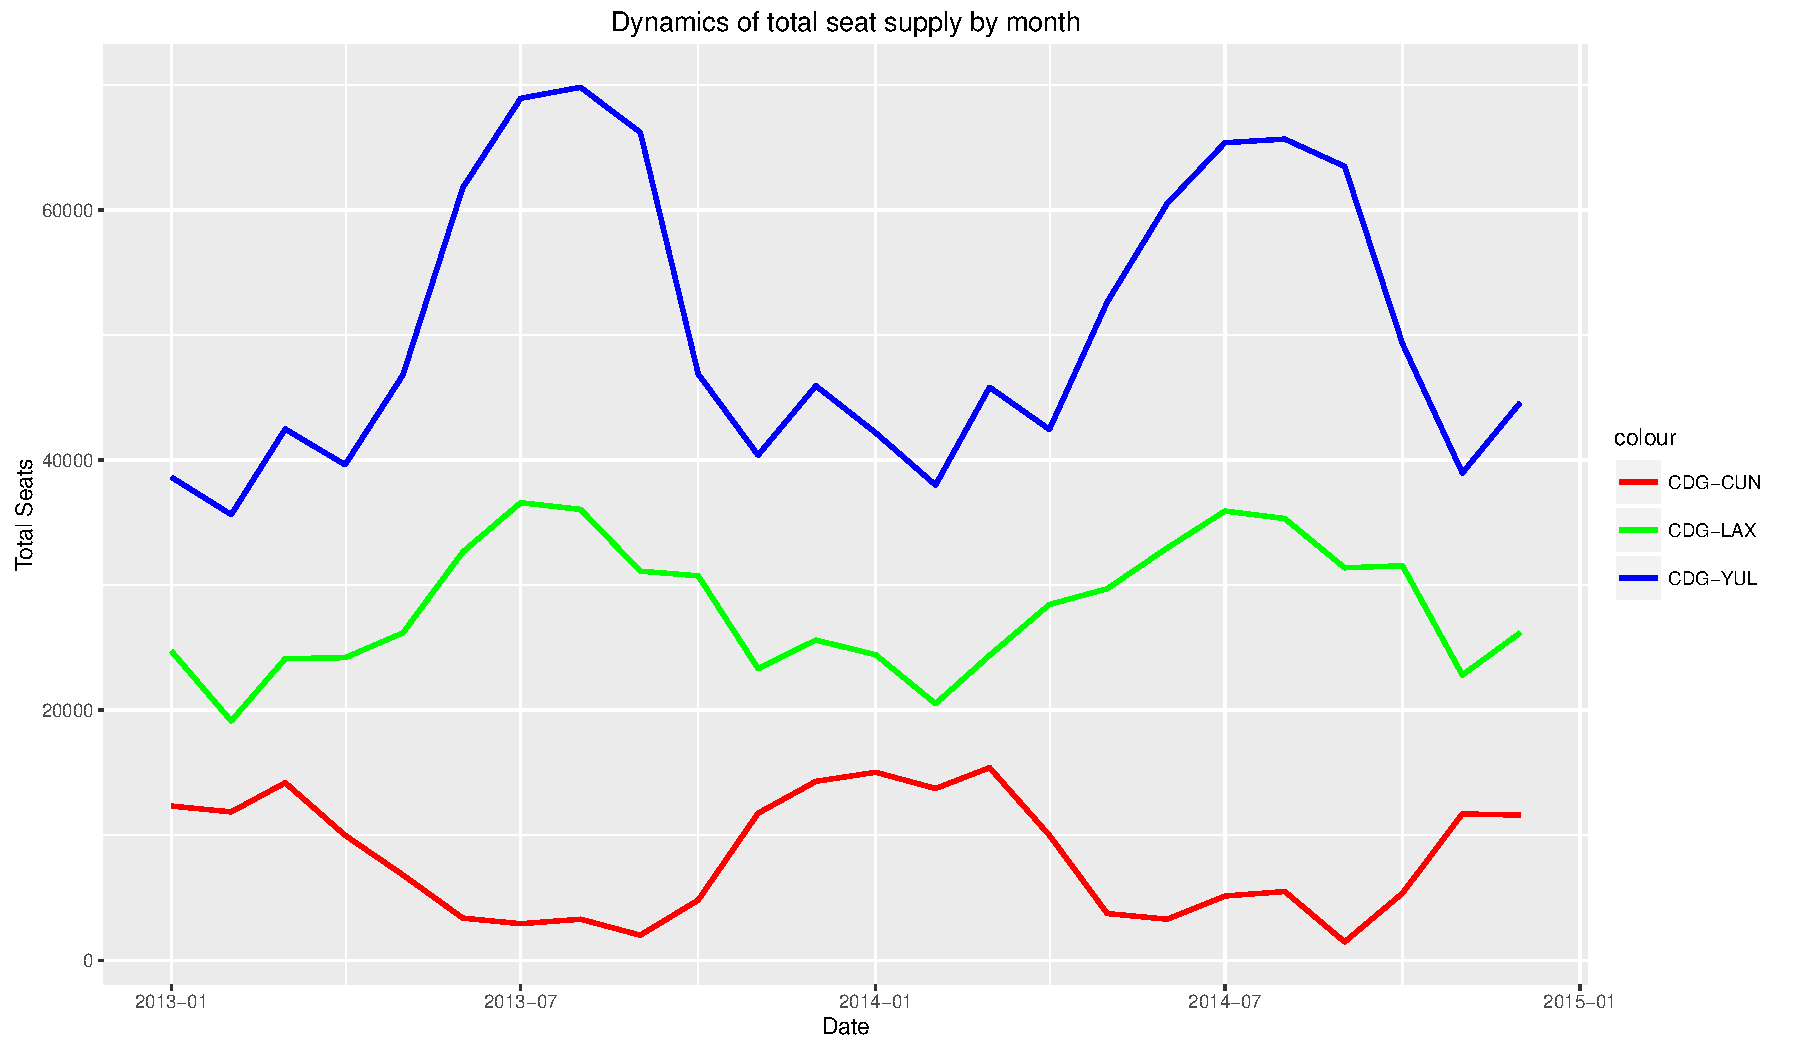
\includegraphics[width=120 mm]{Rplot07.pdf}
\label{season}
\end{figure}
\tab As it could be seen from the figure \ref{season} there is a clear seasonal trend in all of three routes, however, the pattern is not the same\footnote{Blue line corresponds to the airport pair of Paris-Montréal, green - Paris-Los Angeles, red - Paris-Cancun.}. For CDG-LAX (Charles de Gaulle -- Los Angeles Airports), CDG-YUL (Charles de Gaulle -- Montréal Airports) routes we see that seats surge dramatically for summer periods with peaks in July-August, whereas for CDG-CUN (Charles de Gaulle -- Cancun Airports) the highest points comes in December-January. This is not a surprising fact, people travel from Paris to Los Angeles and Montréal in summer period, whereas destination Paris-Mexico is the more favorable for tourism during winter. \\
\tab Seasonality will be controlled in this study by introducing monthly dummy variables\cite{Hsiao}. 
\\
\tab The other potential problem is the trending of independent variables. Overall, there is an annual increase in passenger traffic, as shown in figure \ref{traffic}: 
\begin{figure}[h!]
\centering
\caption{Growth of passenger flow}
\label{traffic}
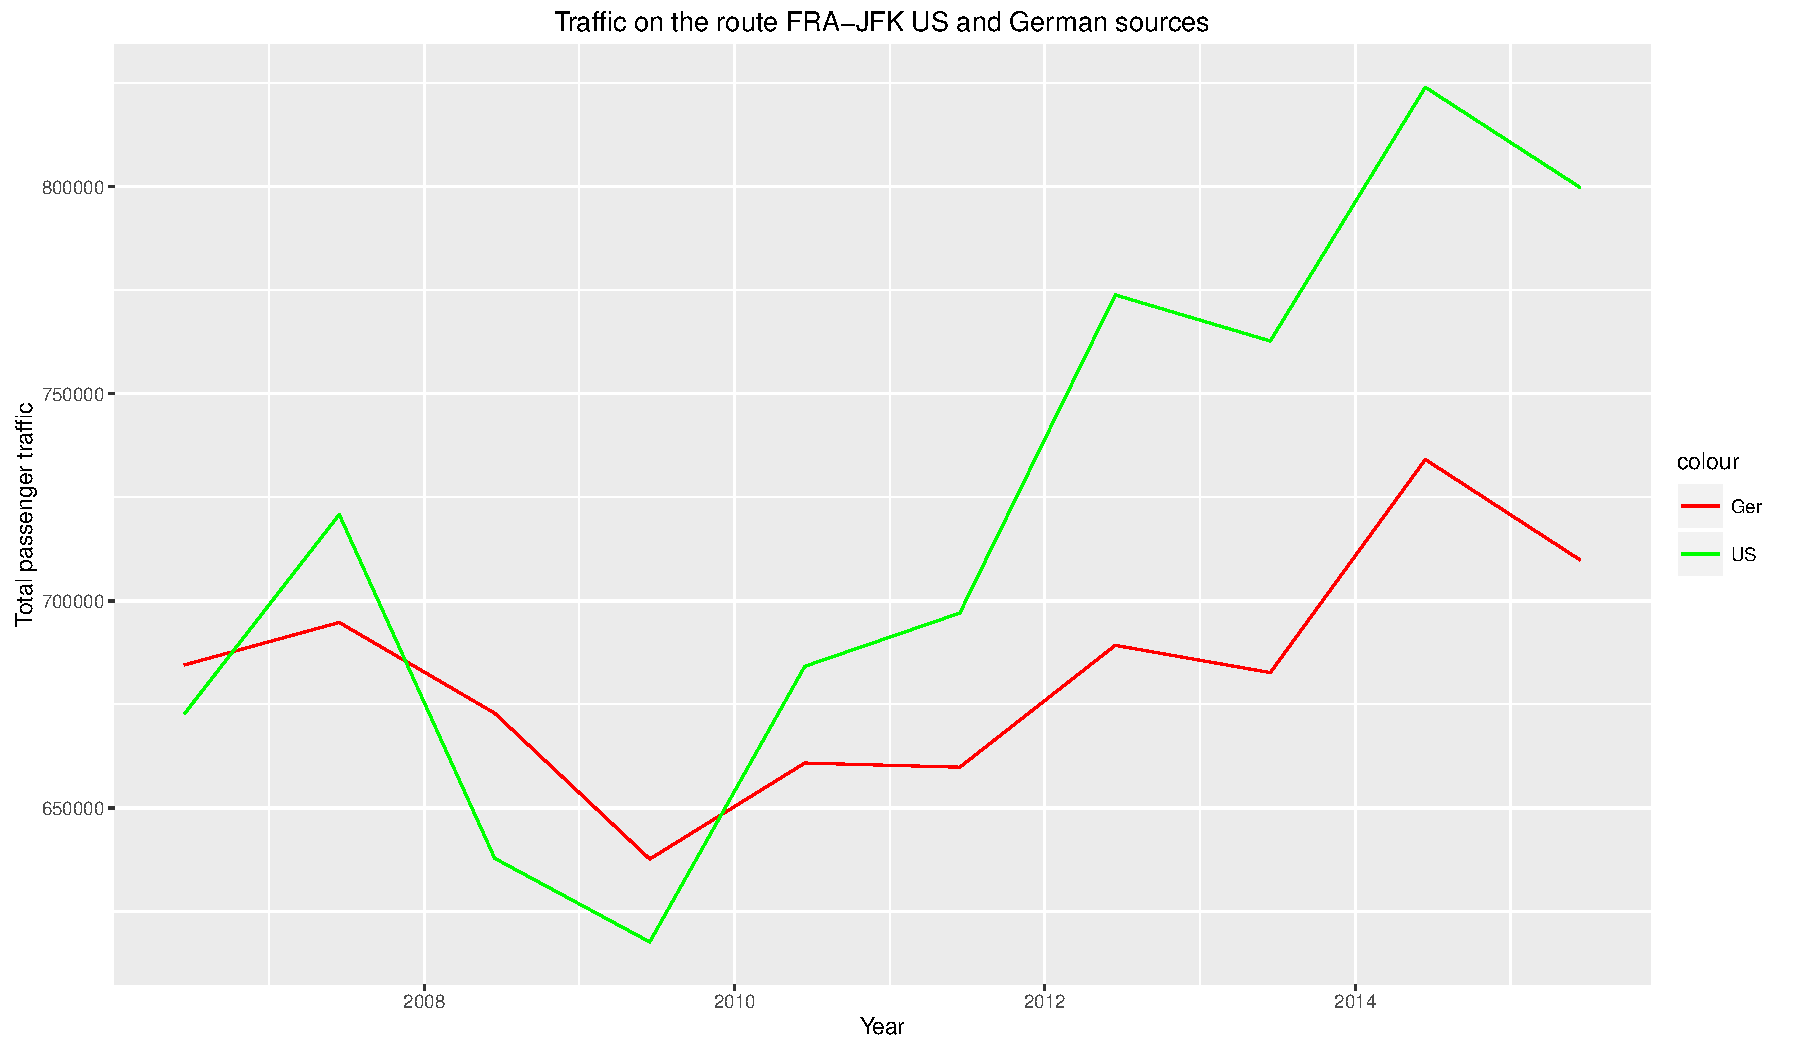
\includegraphics[width=120 mm]{traffic1.pdf}
\end{figure}
\\
\tab Despite the shock in 2007 to 2009 on figure \ref{traffic} due to global financial crisis, there is an upward trend, which is consistent with predictions of scholars that in future passenger flow will continue to increase. Therefore, in our model we will control for special events and shocks using dummy variables for years 2008, 2009 and 2010.\\ 
\tab In total there are 151 airport-to-airport routes on which A-380 aircraft operates. Due to its size, A-380 is designed for long-haul routes with high demand. A long-haul route \cite{seatconfig} is considered to be a non-stop fly with distance greater than 2000 km. Therefore, after conducting the qualitative analysis of the routes, we decided to live only routes that correspond to the definition of long-haul routes. Therefore, 30 routes with distance less than 2000 km were removed from our data set. The airlines on these 30 routes did not use A380 on the regular basis, these were rather exceptional cases, which could potentially be for airlines' experimental purposes. We observe the data on monthly bases for the last 10 years on 121 routes. In total it constitutes N=35,371 observations. The descriptive statistics of the data set is presented in table \ref{sumstat}:
\begin{table}[!htbp] \centering 
  \caption{Descriptive Statistics of variables} 
  \label{sumstat} 
  
\begin{tabular}{@{\extracolsep{5pt}}lccccc} 
\\[-1.8ex]\hline 
\hline \\[-1.8ex] 
Statistic &  \multicolumn{1}{c}{Mean} & \multicolumn{1}{c}{St. Dev.} & \multicolumn{1}{c}{Min} & \multicolumn{1}{c}{Max} \\ 
\hline \\[-1.8ex] 
Distance in km & 6,147.693 & 3,090.971 & 1,985 & 13,802 \\ 
Flight frequency & 54.784 & 51.929 & 1 & 548 \\ 
Log of population & 15.383 & 1.084 & 12.899 & 17.453 \\ 
Number of companies  & 4.268 & 2.911 & 1 & 17 \\ 
Ratio of weight transported by A380  & 0.086 & 0.242 & 0.000 & 0.983 \\ 
Competitors' ratio of weight transported by A380 & 0.084 & 0.197 & 0.000 & 0.975 \\ 
Log of annual traffic$^{*}$ & 13.492 & 0.805 & 1.099 & 15.231 \\
\hline \\[-1.8ex] 
{\textit{Notes}: N=35,371, N$^{*}$=33,983}
\end{tabular} 
\end{table}


\tab As it could be seen from table \ref{sumstat}, the mean distance of the route - 6147 km. The average frequency per airline serving the route is 54 flights per month. On average there are 4 competitors on the route, however, there are routes that are entirely supplied by a single carrier. \\
\tab In this specification we are interested to test the two proxy for demand - logarithm of population and annual route traffic, which was collected from the ENAC autonomous database. However, out of 121 long-haul routes, traffic data is available only for 118. The elimination of three routes decreased the number of observations to N=33,983\\ 
\tab The qualitative exploration of the data  indicates the presence of  heterogeneity in our data set. The issue with the heterogeneity is that regular OLS cannot account for differences across groups or time. The figure \ref{hetyears} represents the plot of the mean value of frequency per period from 2010 to 2015 with blue range indicating -- 95\% confidence interval. From this graph we can deduct that there is a slight upward trend and the mean value of frequency changes over time. Even though this graph depicts only mean values, it provides the rough intuition which show the clear seasonality in the data as well as slightly upward trend.
\begin{figure}[ht!]
\centering.
\caption{Heterogeneity in time series}
\label{hetyears}
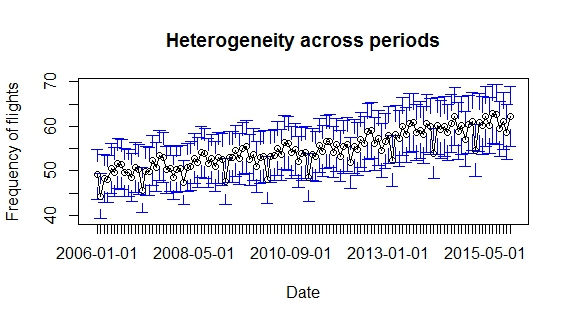
\includegraphics[scale = 0.5]{Rplot.jpeg}
\end{figure}
\tab The figure \ref{density} is a density plot of frequency of flights. We see that the most common frequency is between 0 and 50. The diagram is skewed to the right with the highest frequency of 300 per month.

\begin{figure}[ht!]
\centering
\caption{Density plot of frequency of flights}
\label{density}
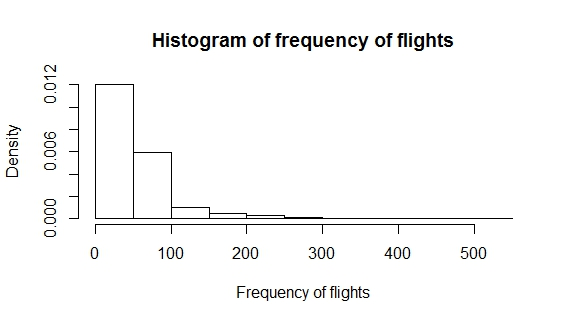
\includegraphics[scale = 0.5]{hist.jpeg}
\end{figure}

\tab Therefore, the visual inspection of the data suggests the presence of heterogeneity in the data. Thus, in order to account for individual-specific effects, it is a common practice in econometrics to use Fixed Effect model, where the individual-specific effects, which cannot be explained by the independent variables, are subtracted. 
\section{Test and Selection of the model}
From the visual inspection of the data, it could be seen that airline data contains time-invariant latent effect that might be specific to route or airline company

General model with individual effect has the following specification \cite{book}: 
\begin{equation} \label{eq:2}
y_{it} = \boldsymbol{x_{it}\beta}  + \alpha_i+ \epsilon_{it} 
\end{equation}
where $\alpha_i$ is an individual unobserved heterogeneity and $u_{it}$ is an idiosyncratic error. Depending on the model specification $\alpha_i$ is interpreted as random or fixed effect \cite{book}. These types of models provide consistent estimation under the strict exogeneity condition, which restricts the effect of independent variables on $y_{it}$ conditional on the unobserved effect $\alpha_i$: 
\begin{equation} \label{eq:3}
E(y_{it}\mid\boldsymbol{x_{it}}, c_i)=\boldsymbol{x_{it}\beta} +c_i
\end{equation}
In terms of idiosyncratic errors this condition is equivalent to the following assumption: 
\begin{equation} \label{eq:4}
E(u_{it}\mid\boldsymbol{x_{it}})=\boldsymbol{0}
\end{equation}
If this assumption does not hold, the common treatment of panel data cannot by applied. The fixed/random effect model due to unobserved heterogeneity will be a starting point in statistical inference. It is one of the most popular approach for estimation of non-dynamic panel regressions. The 

Below is the description of model, which was tested with panel data using pooled OLS, fixed and random effect specification. The choice of the model is based on the test results described further. 

\begin{equation} \label{eq:5}
\begin{split}
FREQ_{ijt} =& \beta_0 + \beta_1NUMBCOMP_{it} + \beta_2LOGPOP_{it}  \textit{ (or } \beta_2LOGTRAF_{it}\textit{) }\\ &+\beta_3RATIO380_{ijt}+\beta_4COMPRATIO380_{ijt}\\ &+\beta_5DUMMY2008_{ijt}+\beta_6DUMMY2009_{ijt} + \beta_7DUMMY2010_{ijt} \\ 
&+\beta_8FEB_{ijt}+\beta_9MAR_{ijt}+\beta_{10}APR_{ijt}+\beta_{11}MAY_{ijt}\\ &+\beta_{12}JUN_{ijt}+\beta_{13}JUL_{ijt}+\beta_{14}AUG_{ijt}+\beta_{15}SEP_{ijt}\\
&+\beta_{16}OCT_{ijt}+\beta_{17}NOV_{ijt}+\beta_{18}DEC_{ijt}+\alpha_i+\epsilon_{ijt} 
\end{split}
\end{equation}
where \\ 
$FREQ$ is the frequency of flights supplied by airline $j$ on the route $i$ per month $t$\\ 
$NUMBCOMP$ is the number of companies that operate on the route $i$ in the period $t$. This variable\\  \tab is used to account   for the structure of competition on the market. The other competition \\  \tab measurements, such as HHI, do not exhibit sufficient variation and thus were excluded  \\
$LOGPOP$ is the logarithm of population in the departure airport of the route $i$ per year, \\ \tab proxy for demand for airline services\\
$LOGTRAF$ is the logarithm of two-way annual traffic on the route, another proxy for demand \\  \tab for airline services. These two demand proxies will be tested separately to test the robustness of \\ 
\tab  the model\\
$RATIO380$ is the ratio of maximim total weight (seats and cargo converted to kg) transported by aircraft \\ 
\tab A380. It reflects the intensity of utilization of A380 on the route with respect to other aircraft types\\ 
\tab to total weight transported by all type of aircraft. \\
$COMPRATIO380$ is the competitors' ratio of total weight (seats and cargo converted to kg) transported \\ 
\tab by aircraft A380 on the route to total weight transported by all type of aircraft. It  reflects \\ 
\tab the intensity of utilization of A380 by competitors on the route with respect to other aircraft types. \\
$DUMMY2008$ is the dummy variable indicating year 2008 period of financial crisis\\
$DUMMY2009$ is the dummy variable indicating year 2009 period of financial crisis\\
$DUMMY2010$ is the dummy variable indicating year 2010 period of financial crisis\\ 
$FEB$ - $DEC$ are the dummy variables indicating the month of the year 
\subsection{Testing the validity of model}  

% latex table generated in R 3.3.1 by xtable 1.8-2 package
% Mon Aug 29 11:38:40 2016
\begin{table}[ht]
\centering
\label{test}
\begin{tabular}{rll}
 & Test & Results \\ 
  \hline

1 & Lagrange Multiplier Test -  (Breusch-Pagan): & t(1) = 5229133.77, p $<$ .001, d = 5229133.77 \\
2 & Lagrange Multiplier Test - time effects (Breusch-Pagan): & t(1) = 1366.60, p $<$ .001, d = 1366.60 \\
3 & Hausman Test for FE or RE models: & t(18) = 843.41, p $<$ .001, d = 273.64 \\ 
4 & Augmented Dickey-Fuller Test: & t(1) = -14.66, p = .010, d = -14.66 \\ 
5 & Breusch-Godfrey test for serial correlation in panel models: & t(1) = 26224.48, p $<$ .001, d = 26224.48 \\ 
6 & Breusch-Pagan test for heteroskedasticity: & t(124) = 109891.60, p $<$ .001, d = 13900.31 \\ 
\end{tabular}
\end{table}

The table \ref{test} presents a list of tests that were performed to evaluate the validity and justify the final specification of the model. \\ 
\tab The first Breusch-Pagan Lagrange-Multiplier for random effects test helps to decide whether or not there is a panel effect. Even though we qualitatively concluded that there is heterogeneity across groups and time, this test allows to provide the qualitative justification. The null hypothesis is that there is no variance across individuals \cite{book}:
$H_0: \sigma_0=\sigma_1=...=\sigma_n=0$. However, as we can see, the corresponding p-value is lower than 0.001, thus, we reject null hypothesis in favor of alternative, indicating significant heterogeneity across entities.  \\ 
\tab The next test is also Lagrange Multiplier test for time effects. As we can see from p-value, which is lower than 0.001, there is a strong evidence for using time fixed effects. These two tests allowed to reject the simple OLS model in favor of fixed or random effect and establish the significant influence of time series dimension of panel structure.    \\ 
\tab The next test is the Hausman test for fixed effect vs random effect estimation. 
In this specification we have the following generalization of the model: 
\begin{equation} \label{eq:6}
y_{it} = \beta_0 + \beta_1x_{it} + \alpha_i + u_{it}
\end{equation}
where $y$ is the independent variable, $x$ is the dependent variable, both varying for individuals across time and some unobserved factor $\alpha_i$. The random effect model along with strict exogeneity (\ref{eq:4}) assumes that there is no covariance between unobserved effect $\alpha_i$ and independent variables: $Cov(\alpha_i, x_{it})=0$. If this condition holds, then both random effect and fixed effect estimators are consistent, with random effect estimator being the most efficient one \cite{book}. If this condition does not hold, then random effect is no longer consistent. The null hypothesis of the Hausman test is $H_0:Cov(\alpha_i, x_{it})=0$. From the p-value of the test, we reject null hypothesis and conclude that random effect model is not appropriate, since unique errors are correlated with the independent variables. \\ 

\tab Fixed effect approach removes the unobserved effect by preserving time-demeaned data \cite{book}, however; the explanatory variables that are constant over time are removed from equation, therefore the variable such as route distance, which may play significant role on airline policy does not enter the equation. The general equation of fixed effect is below, where $\bar{y}$ is the individual mean value: 
\begin{equation}
y_{it}-\bar{y}_i = \beta_1(x_{it}-\bar{x_i}) +u_{it}-\bar{u_i}
\end{equation}

Under the earlier mentioned strict exogeneity assumption \ref{eq:4}, where each error term is uncorrelated with explanatory variables across all time periods, the fixed effect regression provides an unbiased estimation.


\tab The next is Augmented Dickey-Fuller test to verify that the independent variables are coming from the same data generating process in all time periods, which means that the independent variable $x$ in period $t$ follows the same process as in period $t+1$ and other periods. There are three conditions of the stationary process \cite{book}:
\begin{itemize}
\item $E(x_{t}) = \mu$ 
\item $Var(x_{t}) = \sigma^2$
\item $Cov(x_t, x_{t+h}) = f(h)\neq g(t) $
\end{itemize}
The first is that the expected value of $x_t$ is equal to  constant $\mu$. The second conditions is that variance of $x_t$ is constant. The last is that covariance between $x_t$ and $x_{t+h}$ is a function, independent of time. Therefore, if we want to establish the linear relationship between $y_t$ and $x_t$, the stationary of time series is a necessary condition. Moreover, the presence of stationary data allows to ensure the application of Law of Large Numbers and Central Limit Theorem. The idea in Augmented Dickey-Fuller test is to run the following regression \cite{book}: 
\begin{equation}
\Delta y_t = \alpha + \delta y_{t-1} + \epsilon{t} 
\end{equation}
where the null hypothesis is that there is a unit-root: $H_0: \delta = 0$. In the table the value of p-statistics is less than 0.01, therefore, we reject null hypothesis in favor of alternative hypothesis for stationarity of time series. \\
\tab The following test is the Breusch-Godfrey test for serial correlation or in equivalent terms autocorrelation. The definition of serial correlation is that the covariance between the two error terms is not equal to zero\cite{book}: $Cov(u_{it}, u_{st'}) \neq 0$, $\forall$ $i$, $s$, $t$, $t'$. The presence of serial correlation leads the estimators to be no longer best linear unbiased estimators, there are other estimators that are more efficient with lower variance. In the table the p-value for Breusch-Godfrey is lower than 0.001, therefore, there is a strong evidence against $H_0:Cov(u_{it}, u_{st'})=0$, in favor of alternative hypothesis, justifying the presence of serial correlation. Therefore, our next approach is to construct a model with serial correlation robust inference. \\
\tab The last test is Breusch-Pagan test for heteroskedasticity. In the presence of homoskedastic errors, the following condition holds:  $H_0:Var(u_{it}\mid x_{it}) = \sigma^2$, the variance of the error terms given the independent variables is constant, whereas under heteroskedasticity it is a function of the regressors:  $Var(u_{it}\mid x_{it}) = \sigma^2f(x_{it})$. In the test table p-value is less .001, indicating the presence of heteroskedasticity. Therefore, the robust errors will be provided accounting for non-constant variance. 

\subsection{Correcting for serial correlation: AR(1) process}
The presence of serial correlation indicates that the usual test statistics is no longer valid\cite{book}. If we consider that errors follow the AR(1) process: 
\begin{equation}
u_{it} = \rho u_{it-1}, \textnormal{for all t} 
\end{equation}
then the variance of error term is: 
\begin{equation}
Var(u_{it})= \frac{\sigma_e^2}{1-\rho^2}
\end{equation}
One of the measures to tackle autocorrelation is to change model by quasi-differencing: 
\begin{equation}
y_{it} - \rho y_{it-1}= (1-\rho)\beta_0 + \beta_1(x_{it}-\rho x_{it-1}) + (u_{it}-u_{it-1}) 
\end{equation}
The error terms of the above equation are not serially correlated. The estimator $\rho$ is the sample autocorrelation estimate of residuals, obtained by regression and iteration. The quasi-differenced coefficients of the above equation are the special case of Feasible GLS estimator. In this paper, we will use Prais-Winsten method instead of Cochrane-Orcutt, since the last uses the notion of lag and loses the first observation. Moreover, we will apply heteroskedasticity robust errors. 

\section{Results}

\begin{table}[!htbp] \centering 
  \caption{Model Regression} 
  \label{regres} 
\scalebox{0.7}{
\begin{tabular}{@{\extracolsep{5pt}}lcccc} 
\\[-1.8ex]\hline 
\hline \\[-1.8ex] 
 & \multicolumn{4}{c}{\textit{Dependent variable: frequency of flights}} \\ 
\cline{2-5} 
\\[-1.8ex] &  (1) & (2)& (3)& (4) \\ 
\\[-1.8ex] & \textit{Robust FE} & \textit{Prais-Winsten} &\textit{Prais-Winsten} &\textit{Prais-Winsten}  \\  
 & \textit{estimator} & \textit{estimator} & \textit{estimator}& \textit{estimator} \\  %\multicolumn{3}{c}{\textit{linear}} 
\\[-1.8ex] & 121 routes & 121 routes & 118 routes & 118 routes\\ 
\hline \\[-1.8ex] 
 Constant & -- & $-$85.177$^{***}$ & $-$341.605$^{***}$ & $-$191.755$^{***}$ \\ 
  &  & (30.24)& (87.85) & (52.52) \\ 
  & & & & \\ 
 Number of companies & 2.048$^{***}$ &  0.279$^{**}$ & 0.269$^{**}$ &  0.268$^{**}$ \\ 
  & (0.578) & (0.12) & (0.12) & (0.12) \\ 
  & & & & \\ 
 Log of population & 66.895$^{***}$ &  7.758$^{***}$ & 3.287 & -- \\ 
  & (7.878) &  (2.00) & (3.82)  &  \\ 
  & & & & \\ 
 Log of annual traffic on route & -- & -- & -- & 0.287$^{**}$ \\ 
  &  &  &   & (0.14) \\ 
  & & & & \\   
  Share of A380 tonnes supplied by airline & $-$7.540$^{***}$ & $-$4.926$^{***}$ & $-$4.960$^{***}$ & $-$4.958$^{***}$ \\ 
  & (1.637) & (0.69) & (0.70) & (0.70) \\ 
  & & & & \\ 
 Share of A380 tonnes supplied by competitors & $-$7.053$^{***}$ &  1.468$^{**}$ & 1.207$^{*}$ & 1.214$^{*}$ \\ 
  & (1.909) & (0.475) & (0.476) & (0.476) \\ 
  & & & & \\ 

 fixed effect 2008 & $-$0.790 &    0.065& 0.068 &  0.090  \\ 
  & (0.548) & (0.24) & (0.24) & (0.24) \\ 
  & & & & \\ 
fixed effect 2009 & $-$1.621$^{***}$ &   $-$0.570$^{**}$ & $-$0.580$^{**}$ & $-$0.571$^{***}$ \\ 
  & (0.615) & (0.26) & (0.27) & (0.27) \\ 
  & & & & \\ 
fixed effect 2010 & $-$1.941$^{***}$ &  $-$0.293 & $-$0.296 & $-$0.293 \\ 
  & (0.579) & (0.20) & (0.20) & (0.20) \\ 
  & & & & \\ 
Feb & $-$5.097$^{***}$ & $-$5.343$^{***}$ & $-$5.195$^{***}$ & $-$5.200$^{***}$ \\ 
  & (0.271) & (0.12) & (0.11) & (0.11) \\ 
  & & & & \\ 
 Mar & $-$0.128 & 0.438$^{**}$ & $-$0.456$^{**}$ & $-$0.466$^{**}$ \\ 
  & (0.143) & (0.15) & (0.15) & (0.15) \\ 
  & & & & \\ 
 Apr & $-$0.577$^{**}$ & $-$1.234$^{***}$ & $-$1.211$^{**}$ & $-$1.226$^{**}$ \\ 
  & (0.261) & (0.18)  & (0.18) & (0.18) \\ 
  & & & & \\ 
 May & 1.099$^{***}$ & 0.273 & 0.237 & 0.216 \\ 
  & (0.345) & (0.19) & (0.19) & (0.19) \\ 
  & & & & \\ 
 Jun & $-$0.128 & $-$1.087$^{***}$ & $-$1.061$^{***}$ & $-$1.088$^{***}$ \\ 
  & (0.394) & (0.19) & (0.19) & (0.19) \\ 
  & & & & \\ 
 Jul & 2.401$^{***}$ & 1.398$^{***}$ & 1.333$^{***}$ & 1.301$^{***}$ \\ 
  & (0.422) & (0.19) & (0.19) & (0.19) \\ 
  & & & & \\ 
 Aug & 2.591$^{***}$ & 1.406$^{***}$ & 1.339$^{***}$ & 1.302$^{***}$ \\ 
  & (0.420) & (0.19) & (0.19) & (0.18) \\ 
  & & & & \\ 
 Sep & 0.043 & $-$1.153$^{***}$ & $-$1.142$^{***}$ & $-$1.185$^{***}$ \\ 
  & (0.389) & (0.18) & (0.18) & (0.18) \\ 
  & & & & \\ 
 Oct & 1.420$^{***}$ & 0.226 & 0.192  &0.144 \\ 
  & (0.314) & (0.17) & (0.18) & (0.17) \\ 
  & & & & \\ 
 Nov & $-$0.808$^{***}$ & $-$2.129$^{***}$ & $-$2.139$^{***}$ & $-$2.193$^{***}$ \\ 
  & (0.201) & (0.14) & (0.14) & (0.13) \\ 
  & & & & \\ 
 Dec & 1.588$^{***}$ & 0.121 & 0.043 & $-$0.016 \\ 
  & (0.219) & (0.09) & (0.11) & (0.09) \\ 
  & & & & \\ 

\hline \\[-1.8ex] 
Observations & 35,371 & 35,371 & 33,983 & 33,983 \\ 
Adjusted R$^{2}$ & 0.182 & 0.161 & 0.165 & 0.165 \\ 
DW statistics & <0.001 & 2.264 & 2.264 & 2.264 \\ 
%F Statistic & 440.681 $^{***}$ & 1,695.991$^{***}$ (df = 4; 34903) & 387.493$^{***}$ (df = 18; 35352) & 387.493$^{***}$ (df = 18; 35352) \\ 
\hline 
\hline \\[-1.8ex] 
\textit{Note:}  & \multicolumn{4}{r}{$^{*}$p$<$0.1; $^{**}$p$<$0.05; $^{***}$p$<$0.01} \\ 
\end{tabular} }
\end{table}

In the table \ref{regres} we present the results of the following models: 
\begin{enumerate}
\item The equation 4 using Fixed Effect estimation with robust errors on 121 routes with logarithm of population as a demand proxy, number of observations is 35,371 
\item The equation 4 using iterated Prais-Winsten estimation with heteroskedasticity and autocorrelation robust errors on 121 routes with logarithm of population as a demand proxy,  number of observations is 35,371
\item The equation 4 using iterated Prais-Winsten estimation with heteroskedasticity and autocorrelation robust errors on 118 routes with logarithm of population as a demand proxy, number of observations is 33,983
\item The equation 4 using iterated Prais-Winsten estimation with heteroskedasticity and autocorrelation robust errors on 118 routes with logarithm of annual traffic on the route as a demand proxy. The number of observations is 33,983
\end{enumerate}
\tab As it was mentioned above the total number of routes that are defined as long-haul routes (distance more than 2000 km) is 121 routes. However, only for 118 routes out of 121 there was available data on the annual traffic. Annual traffic and logarithm of population are proxies for airline demand. These two proxies were tested to verify the robustness of the model.  \\ 
\tab For comparison we provided the results of heteroskedasticity-robust Fixed Effect coefficients with serial correlation in column 1 of table 2 . The three following columns are calculated with Prais-Winsten iteration on 121 and 118 routes with different proxies of demand to prove the robustness of our model. As we can see from the table there is a significant difference in the value of the coefficients from Fixed  Effect and Prais-Winsten method. Nonetheless, in most of the cases the variables that are statistically significant under Fixed Effect are also significant under Prais-Winster estimation. Important to notice that the robust errors of Prais-Winsten estimations are consistently higher relative to the value of coefficient than the robust errors of Fixed Effect, which corresponds with the idea of Feasible GLS estimation accounting for serial correlation. The Fixed Effect robust errors generally underestimate the truly existing variation of estimators and, thus should be taken with caution if there is a presence of significant serial correlation as it was in our case.\\ \tab 
In the last row of the table \ref{regres} we can see the value of Durbin-Watson test. The value of DW statistic is asymptotically equal to $DW = 2(1-\rho)$ with $\rho$ being the sample autocorrelation of residuals. Thus, DW=2 indicates no autocorrelation, significantly less than 2 - positive autocorrelation, greater than 2 - negative autocorrelation. As we can see from the results Fixed Effect model exhibits significantly positive serial correlation with p-value less than 0.001. The value of DW statistics for Prais-Winsten estimations is close to 2 indicating that we  corrected serial correlation, and thus, we can reject the initial Fixed Effect model. \\ 
\tab The coefficients of three Prais-Winsten models have same values, except for the variable logarithm of population, which loses its significance if the sample is decreased by three routes. In this model specification, we will not explain the value of the coefficient, the interpretation of which is not straight forward, since $\rho$ represents the ratio, but rather  will focus on the value of the sign, indicating direction of the change in the behavior, in order to identify if there is an anticipated response after the introduction of innovation. The signs of coefficients in this model correspond to the theoretical expected results. The increase in the number of companies increases the competition, leading to increase in frequency of flights. If there is an increase in the population, then it has positive impact on frequency of flights: the higher is the demand, the more often airlines will schedule flights. However, in the third column, which provides Prais-Winsten estimation for 118 routes, in comparison to 121 routes in second column, lacking more than 1000 observations this demand proxy has no longer significant impact. Therefore, with the 118 routes for which we had data on annual traffic, we used it as a proxy of demand, instead of logarithm of population.  As it could be seen, the increase in the annual traffic leads to an increase in frequency of flights. The next variable is the ratio of the usage of A-380  on the route, the innovation, the variable of interest in our model. It has negative sign, indicating that the increase in the ratio of use of A380, decreases the airline own frequency. This is an interesting result, which corresponds with the hypothesis that the increase in the size of aircraft leads to decrease in frequency of flights. Thus, indeed, we see that the companies optimize the passenger demand by increasing the number of seats and decreasing the frequency, and possibly lower level of $CO_2$ emission. The next variable is the ratio of use of A380 by the competitors on the route also provides interesting insights. From the Fixed Effect model we might falsely conclude, that if the competitors increase their ratio of usage of A380, the airline own response is to reduce frequency as well, whereas in fact the Prais-Winsten estimation shows the opposite reaction on the competitors’ behavior.
The spacial competition in airline industry - scheduled hours for the flight departures could provide some insights for the positive sign of the coefficient of the competitors ratio of A380. The schedule of flights could be analized in Hotelling framework with airline location on the 24-hour clock \cite{hotelling}. Consumers are distributed not in distance terms but are located over time. The interpretation of the coefficient is that increase in the competitors' ratio of total tonnes carried by A380 increases airline's own frequency of flight. The availability of additional hour on the flight schedule represents product differentiation in airline market: there is a consumer, who values the availability of flight in a particular hour of day \cite{hotelling}. Thus, firms in order to capture this marginal consumer may have incentive to locate closer to competitors' time in order to capture demand. If the airline company introduced A380 on a route, it leads to the decrease of its own frequency as the coefficient on the ratio of use of A380 suggests. This in turn provides additional free slot on the time-schedule, which provides an incentives to competitors on the route to move closer to the airline company in order to 'steal' customers. 
\\
\tab The other variables are dummies for month and year indicating that, in fact, the financial crisis led to the decrease in frequency of flights. The sign of coefficients on monthly dummies indicate that there is seasonal effect on the frequency depending on summer or winter periods. 
\section{Conclusion}\label{conclusion}
\tab This report presents the overview of activities and results performed during the period of internship at ENAC. The report outlines the main results and conclusions contributed to NECTAR project, which investigates the if use of A-380 on the route leads to the decrease in flight frequency. The models presented is a starting point in the analysis of behavior of airline companies and environmental benefits that operation of A-380 might potentially generate. The results suggest that larger size of aircraft A-380 leads to the reduction in frequency of flights. The next steps are to enhance model by incorporating the fuel cost for all planes and to further study to what extend A-380 can contribute to the evolution of more sustainable air transportation system. 
 
\singlespacing
\newpage
\begin{appendices}
\section{}\label{Appendix}
\subsection{Information about A-380} \label{A380info}
\tab A-380 is the biggest passenger aircraft. By introducing this model Airbus aims to meet the future demand for "more-efficient, cleaner, quieter and smarter" aircraft \cite{Airbus}.  % Add a reference 
With typical 4-class configuration A-380 provides seats for 544 passengers, with possible maximum of 853 people transported at once. 

\subsection{Information about OAG} \label{OAGinfo}
\tab The OAG Schedule analyzer provides the most recent data on the scheduled flights \cite{OAG}. OAG report allows to analyze the routes on which airlines operate aircraft A-380 based on dimensions and metrics responding to the need of the search. Below is the example of data extraction based on the selected criteria. We included into database observations of operating carriers on routes where A-380 was used \footnote{In this example airport-market-pair Frankfurt-John F. Kennedy is illustrated}. We included only one-way observations, since two-way is a multiple of one-way schedule. The observations are collected on monthly basis from January 2005 to December 2015
\begin{figure}[h]
\centering
\caption{OAG interface}
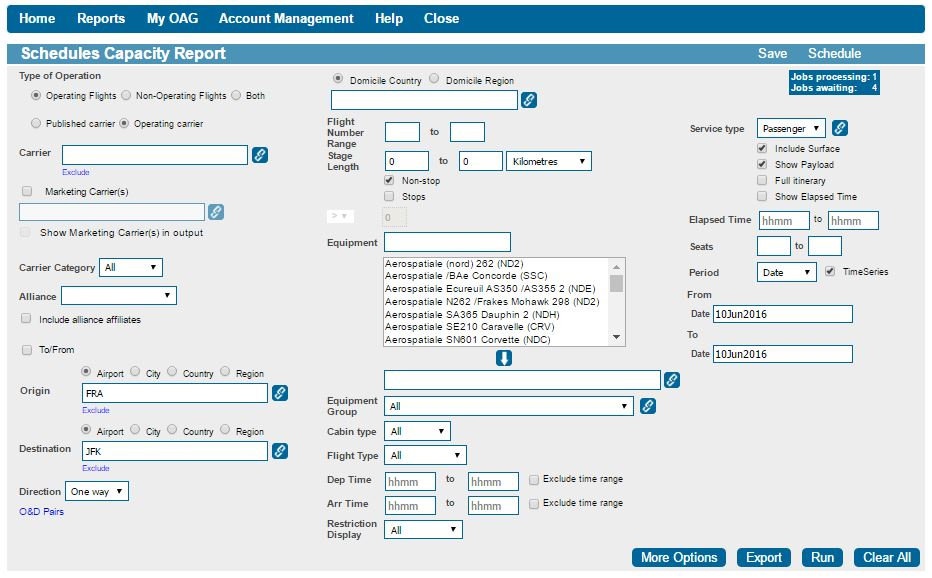
\includegraphics[width=150mm, scale = 1]{OAG.JPG}
\end{figure}
\subsection{BADA: Jet fuel consumption simulation}\label{BADA appendix}
An image below is the example of the simulation with BADA software \cite{BADA}. The first input is the model of aircraft (A-388), the second is the distance flown (6186), the third is the altitude of cruise phase and the last is the total take-off weight, which corresponds to maximum takeoff weight. In the output the data for flight time and fuel consumption is calculated. 
\begin{figure}[h!]
\centering
\caption{BADA software interface}
 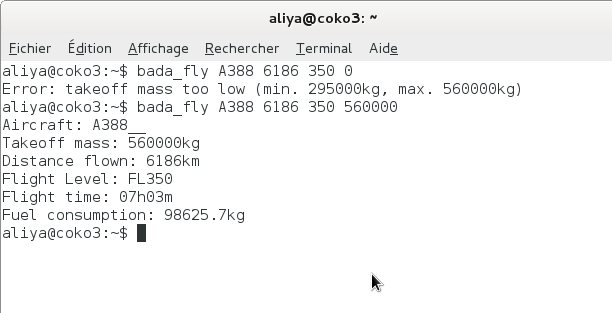
\includegraphics[width=150mm,scale=1]{Cap2.png}\\
\end{figure}
\newpage
\subsection{Literature review summary}

\begin{footnotesize}
\begin{longtable}[h]{|  C{1 cm}  C{1cm}  C{1cm}   C{2cm} C{4cm}  C{5cm}|}
\caption[]{Literature review \label{litreview}}\\
\hline
\textbf{Papers} & \textbf{Airlines} & \textbf{Period} & \textbf{Methodology} & \textbf{Outcome} & \textbf{Why it is useful for us} \\[15mm]  \hline
Wei \cite{Emer1} & 40 airlines from Emerging countries & 2012 & OLS and Logit. Financial performance regressed on innovations and other variables & Technology-based and process- based innovations increase revenues, only process-based increase profit, because the former is costly. Process-based innovations positively affect load factor of airlines. & Ideas for independent variables such as innovation measured as a ratio of aircraft that have this innovation. Control variables that could be tested in our paper are fleet age, airline size, competition expressed as number of destinations to which airline flies. Since larger aircraft is a process-based innovation, we can use conclusions from this paper. \\[15mm] 
Scotti \cite{COEurope} & 18 European airlines & 2000-2010 & OLS model. Efficiency as Biennial Malmquist Luenberger -(BML) index regressed on network characteristics and fuel efficiency & Airlines can boost productivity by introducing bigger aircraft. Increase in load factor increases productivity. Greener aircraft is the primary way to increase environmental productivity & Useful approach to measure environmental productivity. The ideas to test in our model variables that they have used. They came up with the conclusion that larger aircraft help to decrease $CO_2$ emissions \\[15mm] \hline
Hsu and Wen \cite{Fuzzy} & China airlines & 2000 & Fuzzy logic based & Higher load factors leads to airlines determining lower flight frequencies of larger aircraft & Programming approach to model flight frequencies under the competitive equilibrium \\[15mm] 
Devriendt \cite{load} & Airlines in OAG data & Jan - Aug 2001 & Merging demand and supply data to calculate the load factors & The database clearly underestimates load factors. There are potential issues with data sets such as absence of information on non-scheduled flights etc. & They come up with creative approaches to aggregate data. Their approach will be used to manipulate our data and calculate load factors in the routes of our interests \\[15mm] 
Pagovi et al \cite{carbon}& US airlines & first quarter of 2012 & Nested logit model. Game-theoretic approach & After implementation of carbon policy the airlines increase ticket prices leading to demand fall from 2.4 to 21\% depending on carbon fee & They provide good modeling of the airline market (demand and supply) and come up with creative ideas to tackle endogeneity \\[15mm]
Park et al \cite{seatconfig} & Over the world & 2012-2013 & Calculation of fuel burn as a function of aircraft type for a particular route & Fuel efficiency depends on stage length and seat configuration but the larger is the plane the more fuel use decreases & We will use their approach to estimate fuel consumption based on aircraft type and route \\[15mm] 
Zou et al \cite{US} & 15 US jet airlines & 2010 & Ratio-based, deterministic and stochastic frontier approaches & Fuel efficiency improvement can provide cost savings up to 2 and 3 billion US dollars based on different approaches. & They make useful conclusions that we can use for literature review but not the model itself \\[15mm] 
Babic et al \cite{marketshare} & Eastern European Airlines & 2001-2012 & OLS to determine the variables that affect market share and Fuzzy logic to model market share & The two significant variables that affect market share are frequency share and number of competitors per destination at the airport. After training on the data they achieved estimated results close to real & It is useful since it identifies explanatory variables that affect the market share the most \\[15mm] 
Morell \cite{larger} & 7 US airlines &  & Log-Log regression models with dependent variable fuel per seat and independent variable total seats or kg & There is a strong relationship between fuel efficiency and size & This paper is useful since it considers fuel efficiency and aircraft size, we can conduct similar testing with A-380 and compare with other aircraft types \\[15mm] \hline
Miyoshi and Mason \cite{threeMarket} & EU-UK, US-EU& 2004 & Estimation of $CO_2$ using two-stage approach: landing-takeoff and cruise stages & The difference between ratio of covered demand transported by airline and total emission depends on aircraft used, stage length, load factors and cabin configuration & Most of the analysis is done in form of graphs and we can consider their approach for estimation of $CO_2$ emission. \\[15mm] 
Amizadeh et al \cite{commerSixlargest} & 6 EU airlines & 2010-2013 & $CO_2$ emission with respect to different business models & The most $CO_2$ efficient business models are Charters, LCC, Regionals. Despite the increase in traffic the efficiency improves from 1\% to 4.5\% & This paper gave idea to integrate the evolution of traffic flow into the model \\[15mm] 
Li et al \cite{ETSItaly}& 22 airlines & 2008-2012 & SMB and Dynamic DEA models & Efficiency of non-European airlines are much lower than for European ones. The inclusion of airlines into EU ETS forces to improve fuel efficiency to cope with limited carbon emission permits & They nice cope with absence of information and collected it from annual reports, which could be done in our case as well \\[15mm]
Meleo \cite{ETS22} & Italian airlines & 2012-2014 & Formulas for calculating total direct costs, profits and emission & Even if EU ETS carbon fees are 100\% passed onto passengers the final price will increase less than 1\% . Even thought Italian airlines revenues fell it was not due to EU ETS policies & They provide how to compare scenarios if there is an introduction of carbon tax on airlines based on level of emission. This approach could also interesting to consider for A 380 \\[15mm] 
Lu \cite{demandBusiness}& LHR-AMS and LHR-CDG routes &  & Formula for emission calculation, environmental charge and elasticies & Depending on the price elasticies of leisure and business markets the author found different values for  decrease in demand resulting from increase in price. The values range from 0.9 to 7.8\% reduction in demand & This paper gave idea to consider also price elasticies of demand and the type of business models such as network carrier low costers etc. \\[15mm] 
Grimme \cite{economicImpact} & Ryanair, Lufth., Cordon and Air Dolom. & 2008-2012 & Model for future carbon dioxide emission cost of acquiring allowance  and demand & Network carriers can pass more of environmental costs onto passengers than LCC, holiday carriers and regionals. Nonetheless, the financial success of LCC is not likely to be affected & This is a future predictive model, it could be used as a starting point if we will introduce environmental tax in our model \\[15mm] \hline
%\end{tabular}
\end{longtable}
\end{footnotesize}




\end{appendices}


\newpage
\printbibliography
\end{document}
